\documentclass[a4paper,10pt]{jsarticle}

% set length of paper. put 'true' before unit like 31mm = 30truemm.
\usepackage[top=25truemm,bottom=25truemm,left=23truemm,right=23truemm]{geometry}
% set font to 'Times'
\usepackage{newtxtext,newtxmath}
\usepackage[deluxe]{otf}
% multi column
\usepackage{multicol}
\usepackage{color}
\usepackage[dvipdfmx]{graphics}
\usepackage{amsmath,amssymb}
\usepackage{bm} % italic bold (vector)
\usepackage{authblk} % author
\usepackage{fancyhdr} % header and footer
\usepackage{graphicx}
\usepackage{ascmac}
\usepackage{caption}
\usepackage{tikz}
\usepackage{here}
\usepackage{wrapfig} % 画像にテキストを回り込ませる
\usepackage{listings} % source code
\usepackage[version=3]{mhchem} %chemical equatio
\usepackage{titlesec} % relates to section

% settings of section and subsection
\makeatletter
\def\section{\@startsection {section}{1}{\z@}{0.1ex plus -.2ex minus -.2ex}{0.1ex plus .2ex}{\normalsize\textbf}}
\def\subsection{\@startsection {subsection}{1}{\z@}{0.1ex plus -.2ex minus -.2ex}{0.1ex plus .2ex}{\normalsize\textbf}}
\makeatother
%\pagestyle{empty} % ページ番号をなくす
%
%\setlength{\textwidth}{\fullwidth}
%\setlength{\texthight}{40\baselineskip}
%\addtolength{\texthight}{\topskip}
%\setlength{voffset}{-0.55in}
%
% キャプションの設定
\captionsetup[figure]{format=plain, labelformat=simple, labelsep=space, font=footnotesize}
\captionsetup[table]{format=plain, labelformat=simple, labelsep=space, font=footnotesize}
\renewcommand{\figurename}{Figure}
\renewcommand{\tablename}{Table}
%
% setting of source code
\lstset{
    basicstyle={\scriptsize\ttfamily},
    breakindent = 30pt,
    stringstyle={\scriptsize\ttfamily}
}
% document
\begin{document}
% START DOCUMENT
%
% HEADER
\begin{center}
  % title, author
  {\fontsize{14pt}{0pt}\selectfont \textbf{人工流れ星における極超音速希薄流体場の数値解析}\\}
  \vspace{10pt}
  {\fontsize{9.5pt}{12pt}\selectfont $\circ$~林大地 (東北大), Lemal Adrien (ALE Co., Ltd.),\\ \vspace{3pt}
  大西直文, 佐藤慎太郎 (東北大), 蒲池康, 岡島礼奈 (ALE Co., Ltd.)\\}
  \vspace{10pt}
  {\fontsize{12pt}{0pt}\selectfont \textbf{Simulation of the hypersonic rarefied flow environment around an artificial shooting star}\\}
  \vspace{10pt}
  \fontsize{9.5pt}{0pt}\selectfont
  HAYASHI Daichi (Tohoku University), ADRIEN, Lemal (ALE Co., Ltd.),\\ \vspace{3pt}
  OHNISHI, Naofumi, SATO, Shintaro (Tohoku University), Koh Kamachi and Lena Okajima (ALE Co., Ltd.) \\
  \vspace{10.5pt}
  % abstruct
  Abstract \\
  \vspace{-9pt}
\end{center}

\fontsize{9.5pt}{12pt}\selectfont
In order to investigate properties of wake field introduced by an artificial shooting star, numerical simulations ware conducted for thermochemical non-equilibrium flow around a sphere of 1~cm diameter under the calculation condition of the artificial shooting star that Astro Live Experience is working on. A strong shock wave was formed in front of the sphere, and a thermochemical non-equilibrium shock layer was confirmed. The maximum temperature was 22,000~K for translational and rotational temperatures, and 7,000~K for vibrational and electronic excitation temperatures. In addition, local Knudsen numbers and components of drag coefficient were investigated, and it was found that wide region of the wake flow is rarefied, resulting from the small sphere diameter.

\begin{center}
    Key Words : Artificial Meteor, Wake Flow, Thermochemical Non-equilibrium Flow, Rarefied flow\\
    \vspace{10.5pt}
\end{center}

% Main Document Start!
\begin{multicols}{2}
\fontsize{9.5pt}{15pt}\selectfont
\section{緒言}
\par

\section{軌道計算シミュレータの構築}
人工流れ星周りの正確な数値解析を行うにあたり,人工流れ星が移動する流れ場の状況を詳細に把握することは極めて重要である.従って,人工流れ星の放出から,人工流れ星がアブレーションにより質量が無くなるまでを,軌道計算シミュレータを構築することにより再現する.シミュレータは地球中心を原点とする2次元極座標系を考慮した.

また,大気モデルには米国海軍研究所 (the U.S. Naval Research Laboratory, NRL) が公開している NRLMSISE–00~\cite{picone2002nrlmsise} を使用した.
\par

\subsection{軌道計算シミュレータの支配方程式と使用モデル}
軌道上を周回する人工衛星から進行方向後ろ向きに放出された流星源は,放出された地点を遠地点とした楕円軌道に投入される. 放出された流星源の運動方程式は,流星源の位置$\bm{r}$, 速度$\bm{v}$, 質量$m$を用いて式(\ref{eq:equation-of-motion})のように記述される.
\begin{equation}
    \label{eq:equation-of-motion}
    m\dfrac{\mathrm{d}^2\bm{r}}{\mathrm{d}t^2} = -\nabla U(\bm{r}) - \dfrac{1}{2}C_\mathrm{d} S \rho \bm{v}^2\dfrac{\bm{v}}{|\bm{v}|}
\end{equation}
ここで, $C_\mathrm{d}$は抗力係数, $S$は前面投影面積, $\rho$は大気密度であり, $U(\bm{r})$は地球の重力ポテンシャルである.

流星源は大気圏突入時に空力加熱を受け,アブレーションを起こす. アブレーションによる質量減少は式(\ref{eq:mass-by-ablation})で表される. ただし,$C_\mathrm{h}$は単位時間当たりに流星源に供給されるエネルギーのうち,アブレーションに必要となるエネルギーの割合で,熱伝達係数と呼ばれる.$L^*$は流星源が融解,気化及び破砕を含むアブレーションを起こすために単位質量当りに必要になるエネルギーである.
\begin{equation}
    \label{eq:mass-by-ablation}
    L^*\dfrac{\mathrm{d}m}{\mathrm{d}t} = -\dfrac12C_\mathrm{h}S\rho v^3
\end{equation}

さらに,質量の減少に伴って体積および投影面積も変化する.前面投影面積と質量は形状変化係数$\nu$を用いて,式(\ref{eq:area-mass})に従う.ここで,$S_e$と$m_e$はそれぞれ人工衛星から放出された直後の前面投影面積と質量である.
\begin{equation}
    \label{eq:area-mass}
    \dfrac{S}{S_e} = \left(\dfrac{m}{m_e}\right)^\nu
\end{equation}

本研究において,アブレーションによる質量減少過程において形状は変化せず,球形を保ったままであると仮定した.加えて流星源は質量密度が一様であると仮定すれば形状変化係数は式(\ref{eq:shape-coeff})で決まる.これは,球の質量は半径の3乗に比例し,前面投影面積は半径の2乗に比例するためである.
\begin{equation}
    \label{eq:shape-coeff}
    \nu = \dfrac23
\end{equation}

流星源は極超音速で大気圏に突入するため,強い衝撃波が前方に形成され,空力加熱を受ける.この空力加熱は,流動によって行われる対流加熱と,高温により励起された原子が脱励起する際に放出する電磁波によって加熱される輻射加熱に分けられる.流星源は天然のものよりも低速で運動するため,本シミュレータでは対流加熱のみを考慮した.対流加熱による加熱率のモデルには,式(\ref{eq:dkr-model})に示すDetra–Kemp–Riddle~\cite{dkr-model} の推算式(冷壁条件)を用いた.

\begin{equation}
    \label{eq:dkr-model}
	q= \dfrac{110.35}{\sqrt{r}} \left(\dfrac{v}{v_\mathrm{ref}}\right)^{-3.15}\left(\dfrac{\rho}{\rho_\mathrm{ref}}\right)^{0.5}
\end{equation}
ここで,$r$は球半径で,$v_\mathrm{ref} = 7925$~m/s,$\rho_\mathrm{ref} = 1.225$~kg/m$^3$である.この式は軌道から決まる速度と大気密度を用いて対流加熱を見積もることが可能なため,非常に有用である~\cite{nagoya-twins}.

抗力係数$C_\mathrm{d}$は式~(\ref{eq:henderson})に示すように,Henderson~\cite{henderson1976drag}によるモデル式を使用した.
\begin{equation}
    \label{eq:henderson}
%    Cd = \dfrac{0.9+\dfrac{0.34}{M_\infty^2}+1.86\left(\dfrac{M_\infty}{Re}\right)^{1/2}\left[2+\dfrac2{S^2_\infty}+\dfrac{1.058}{S_\infty}\left(\dfrac{T_w}{T}\right)^{1/2}-\dfrac1{S_\infty^4}\right]}{1+1.86\left( \dfrac{M_\infty}{Re} \right)^{1/2}}
    C_\mathrm{d} = \dfrac{0.9+\dfrac{0.34}{M^2}+1.86\left(\dfrac{M}{Re}\right)^{1/2}E}{1+1.86\left( \dfrac{M}{Re} \right)^{1/2}}
\end{equation}
\vspace{-0.7cm}
\begin{align*}
    \mathrm{where}& \\
    E &= 2+\dfrac2{Sa^2}+\dfrac{1.058}{Sa}\left(\dfrac{T_w}{T}\right)^{1/2}-\dfrac1{Sa^4} \\
    Sa &= M\sqrt{\dfrac{\gamma}{2}}
\end{align*}
ここで,$M,\ Re,\ \gamma,\ T$はそれぞれ主流のマッハ数,レイノルズ数,比熱比,温度であり,$T_w$は球の壁面温度である.

また,Prevereaud~\cite{prevereaud2016phd}によると,熱伝達係数$C_\mathrm{h}$は式~(\ref{eq:prevereaud})のようにマッハ数と流星源が受ける加熱率$q$の関数として与えられる.
\begin{equation}
    \label{eq:prevereaud}
    C_\mathrm{h} = \dfrac{2q}{\rho v^3}\dfrac{I_1}{I_2}
\end{equation}
\vspace{-0.7cm}
\begin{align*}
    &\mathrm{where}\\
    I_1 &= \int_0^{\frac{\pi}{2}}\left\{\left( \sin^2\theta + \dfrac{\cos^2\theta}{1+\zeta M^2} \right)\left(\dfrac{\pi}{2} - \theta\right)\cos\theta\sin\theta\right\}\mathrm{d}\theta \\
    I_2 &= \int_0^{\frac{\pi}{2}}\left\{\left( \sin^2\theta + \dfrac{\cos^2\theta}{1+\zeta M^2} \right)\left(\dfrac{\pi}{2} - \theta\right)\cos^2\theta\right\}\mathrm{d}\theta
\end{align*}
    
また,大気の粘性係数はSutherlandの式によって求めた.
\par

\subsection{軌道計算シミューレータの数値計算法と計算条件}
本シミュレータでは,式(\ref{eq:equation-of-motion})と式(\ref{eq:mass-by-ablation})の微分方程式を$r,\dot{r},\theta,\dot{\theta},m$の時間微分について解いた5つの連立微分方程式として4段4次のRunge–Kutta法により数値的に解いた.ただし,従属変数上部のドットは時間微分を表す.

アブレーションにより質量減少が起きるが,その際には質量が$10^{-9}$~kgを下回ると完全に消滅したとして,計算を終了した.

次に,軌道計算シミューレータの初期条件を表~\ref{table:condition}に示す.この初期条件は木村~\cite{kimura2018master}と同様の条件に設定した.

\begin{table}[H]
    \centering
    \label{table:trajectory-init}
    \caption{軌道計算シミューレータにおける初期条件.値は木村~\cite{kimura2018master}の条件と同様に設定した.}
	\begin{tabular}{ll}
	    \hline \hline
	    時刻 & 2020年1月1日 0:0:0(UTC) \\
        初期位置 & W43$^\circ$ N63$^\circ$ 高度375~km \\
        初期速度 & 7330~m/s \\
        流星源密度 & 5000~kg/m$^3$ \\
        流星源形状 & 球, $\phi$ 10~mm \\
        \hline \hline
    \end{tabular}
\end{table}
\par

\subsection{軌道計算シミューレータの結果と先行研究との比較}
初めに,高度に対する大気の密度及び温度分布をFig.~\ref{fig:vs-kimura-rho},Fig.~\ref{fig:vs-kimura-temp}にそれぞれ示す.Fig.~\ref{fig:vs-kimura-rho}から,大気密度は概ね良好な一致を示していると言える.対してFig.~\ref{fig:vs-kimura-temp}に示す大気温度は高度250~km付近で50~K以上の誤差があり,高度120~km以下でも誤差が見られた.120~km以下での温度誤差については,木村~\cite{kimura2018master}では人工衛星から放出される角度も考慮されており,対して本シミュレータは角度が不明だったため初期位置から座標は移動していない.従って高度が下がるほどに座標に誤差が生じ,その座標の誤差によって低高度(120~km)以下での温度に誤差が生じている.また,高高度(150~km以上)の温度誤差について,先程述べた座標の誤差に加えて,太陽条件や地磁気擾乱の活発性を考慮していないことが原因で,温度が低くなっている.

高高度の温度誤差については,輻射加熱には影響するが大気密度が低いため,対流加熱への寄与は小さくアブレーションもほとんど起こらないため,許容できる誤差であると言える.また,低高度での温度誤差については,誤差率が小さいため許容できるものとした.
\begin{figure}[H]
	\centering
	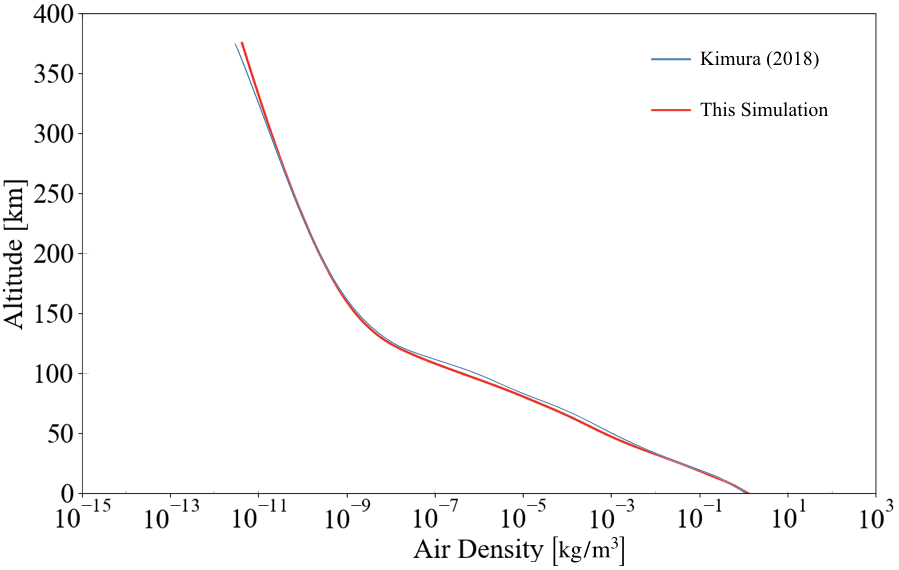
\includegraphics[width=7.5cm]{fig/vs_Kimura/rho}
	\caption{大気密度の結果(赤)と木村~\cite{kimura2018master}の結果(青)との比較.良好な一致を示していると言える.}
	\label{fig:vs-kimura-rho}
\end{figure}
\begin{figure}[H]
	\centering
	\includegraphics[width=7.5cm]{fig/vs_Kimura/temp}
	\caption{大気温度の結果(赤)と木村~\cite{kimura2018master}の結果(青)との比較.高度250~km付近で50~K以上の誤差が確認される.}
	\label{fig:vs-kimura-temp}
\end{figure}

また,Fig.~\ref{fig:vs-kimura-velo}および~\ref{fig:vs-kimura-mass}には軌道計算シミュレータにより得られた速度分布と質量分布をそれぞれ示す.どちらも一見して良好な一致を示し,先程の温度誤差も大きな影響を及ぼさなかったことがこれらの結果からも確認された.Fig.~\ref{fig:vs-kimura-velo}で高度70~km付近で途切れているのは,アブレーションにより燃え尽きたためである.

速度分布を見ると,人工衛星から放たれた流星源は高度100~km付近までは加速するが,それより高度を落とすと,大気層に入り動圧抵抗を受けることで減速に転じていることが確認される.

\begin{figure}[H]
  \centering
  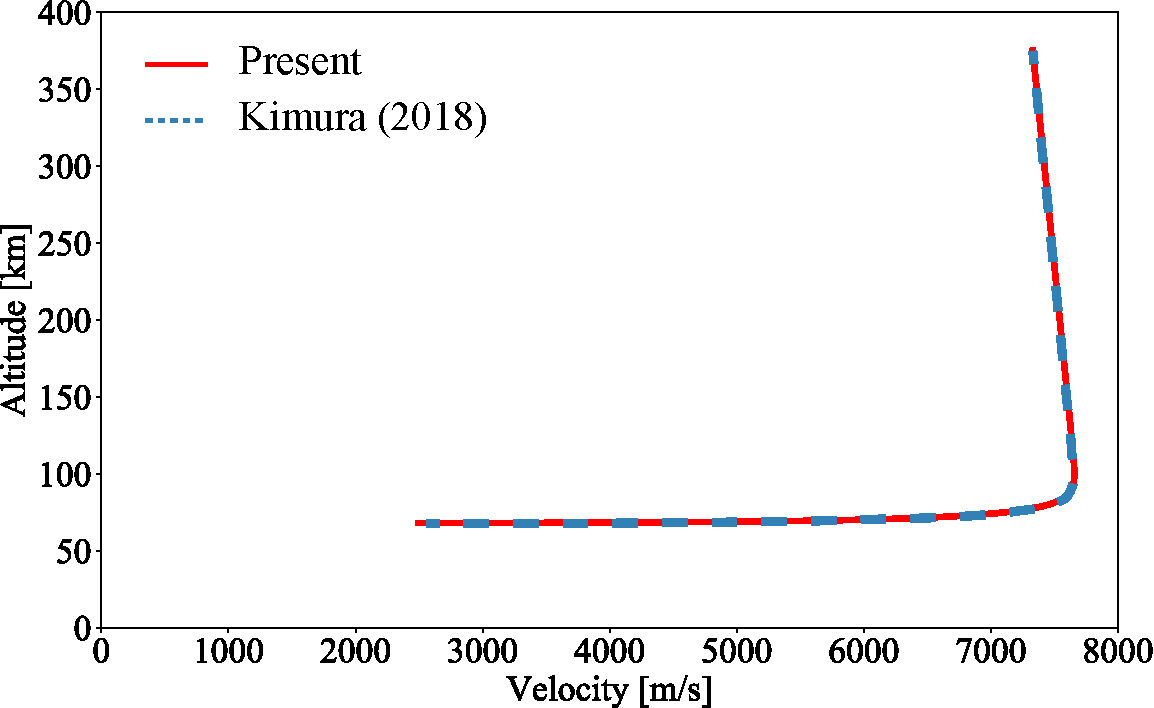
\includegraphics[width=7.7cm]{fig/vs_Kimura/velo}
  \caption{軌道計算シミュレータによる流星源の速度分布(赤)と木村~\cite{kimura2018master}との比較.高度70~km付近で途切れており,アブレーションにより消滅したことが確認される.}
  \label{fig:vs-kimura-velo}
\end{figure}
\begin{figure}[H]
  \centering
  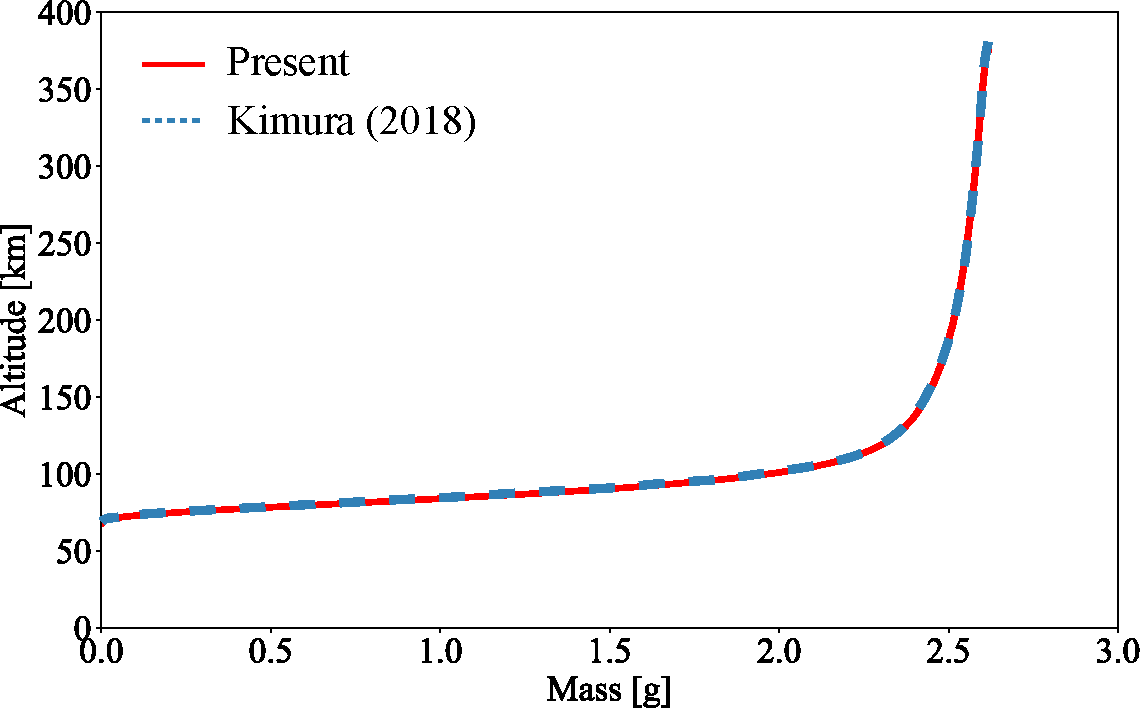
\includegraphics[width=7.7cm]{fig/vs_Kimura/mass}
  \caption{軌道計算シミュレータによる流星源の質量分布(赤)と木村~\cite{kimura2018master}との比較.アブレーションによる質量減少が確認される.特に高度100~km付近から急激に質量減少が起こり,空力加熱を大きく受けている.}
  \label{fig:vs-kimura-mass}
\end{figure}

また,図表は省略するが,マッハ数,レイノルズ数,抗力係数,熱伝達係数などのパラメータもFig.~\ref{fig:vs-kimura-velo}, \ref{fig:vs-kimura-mass}同様に良好な一致を示した.

これらの結果より,構築した軌道計算シミュレータは木村~\cite{kimura2018master}と同様な結果が得られるものとし,シミュレータの結果から流体計算の条件として用いることとした.

Figure~\ref{fig:trajectory-knud}には高度に対するKnudsen数分布を示す.Knudsen数$Kn$は気体の希薄度を示す指標であり,$Kn\ll 1$の領域において連続体近似が可能であり,大きなKnudsen数では流体計算を行うことは不可能である.Fig.~\ref{fig:trajectory-knud}を見ると,高度73~kmにおいて最小Knudsen数である0.99をとっていることが分かる.最小Knudsen数ですら$Kn\ll 1$ではないため流体計算を行うことは難しいと言える.

\begin{figure}[H]
  \centering
  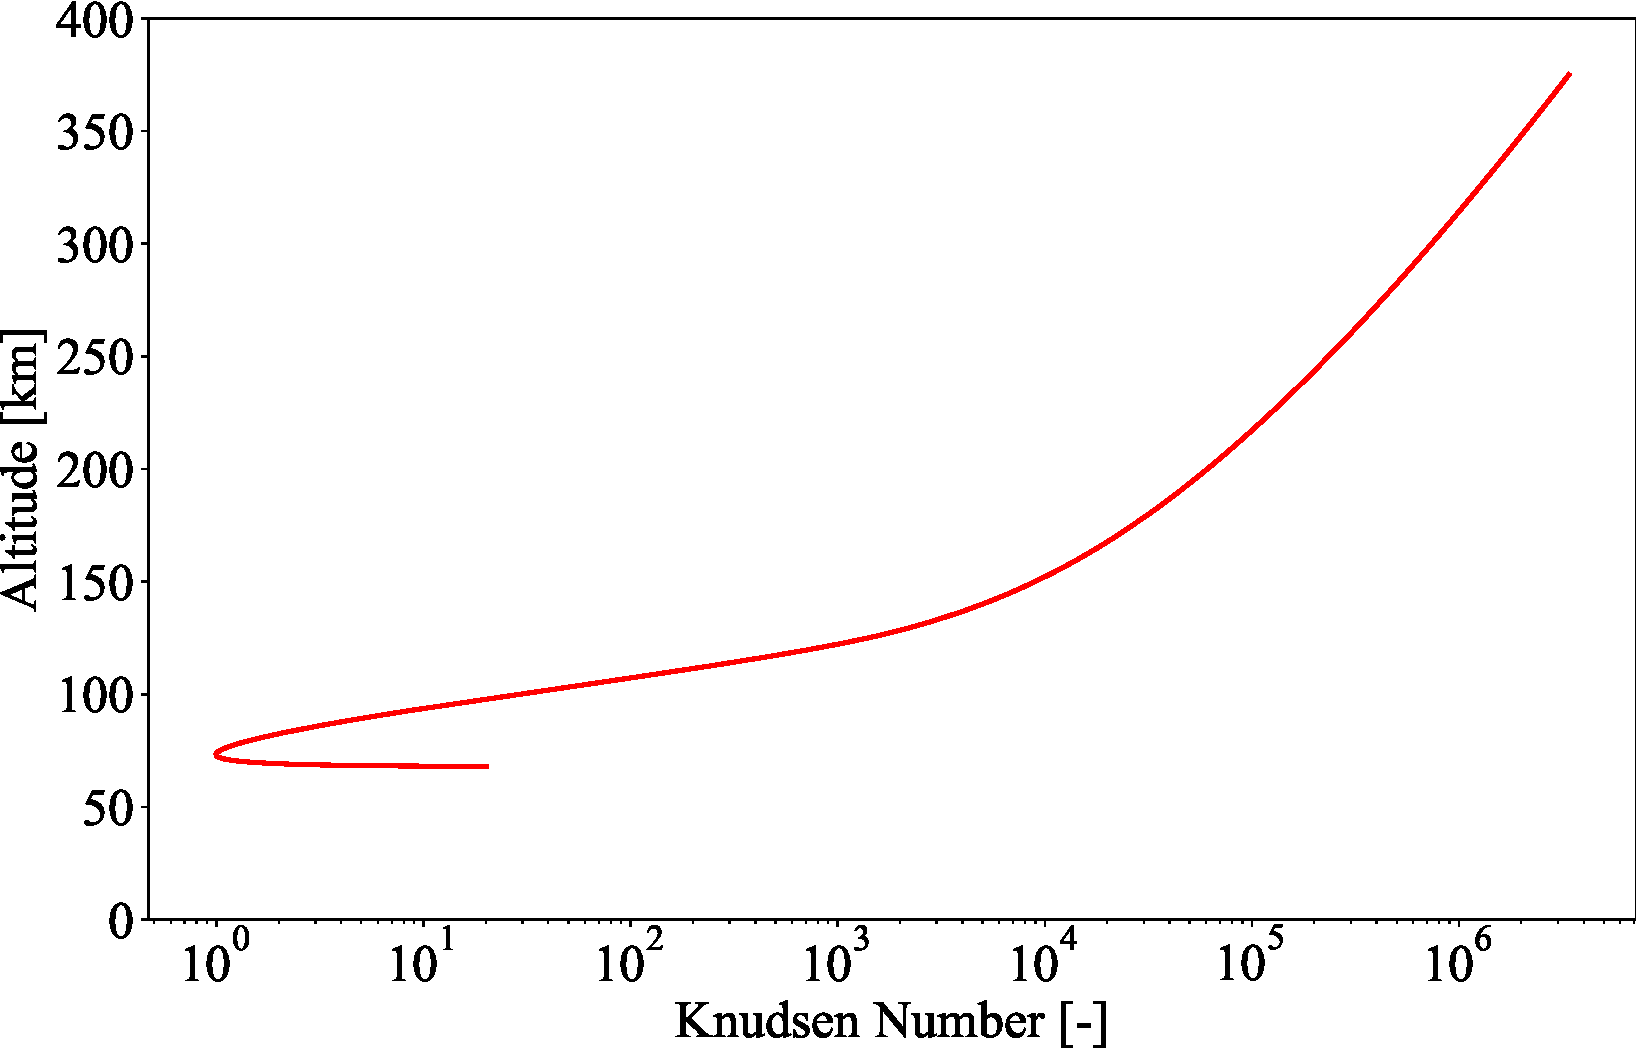
\includegraphics[width=7.7cm]{fig/vs_Kimura/knud}
  \caption{軌道計算シミュレータによるKnudsen数分布.高度73~kmにおいて最小値0.99をとる.軌道上のほとんどの領域でKnudsen数は1を超え,自由分子流に近づいていることが分かる.}
  \label{fig:trajectory-knud}
\end{figure}


\par


\section{数値計算法}
\subsection{流体場の数値計算法}
本研究では,球体周りにおける2次元軸対称流体計算を行う.流れ場の支配方程式は以下に示す2次元軸対称圧縮性Navier--Stokes方程式とする.
 \begin{equation}
 \begin{split}
    \dfrac{\partial \bm{Q}}{\partial t}+\dfrac{\partial \left( \bm{F}-\bm{F}_{\mathrm{vis}} \right)}{\partial x} 
    &+ \dfrac{\partial \left( \bm{G}-\bm{G}_{\mathrm{vis}} \right)}{\partial y} \\
    &+ \dfrac1y\left(\bm{H}-\bm{H}_\mathrm{vis}\right) = \bm{W}
\end{split}
\end{equation}
ここで,$\bm{Q}$は保存量ベクトル,$\bm{F},\,\bm{G}$は対流流束ベクトル,$\bm{F}_\mathrm{vis},\,\bm{G}_\mathrm{vis}$は粘性流束ベクトル,$\bm{H},\,\bm{H}_\mathrm{vis}$は軸対称性から生じる項,$\bm{W}$は生成項ベクトルである.支配方程式を有限体積的に離散化し,数値流束の評価にはAUSM-DVを用いる.空間精度はMUSCL法により2次精度を保持する.

極超音速気流におかれた物体の前方には,強い衝撃波が形成されるために,衝撃層内部では熱化学的な非平衡性を呈す.従って熱化学非平衡性を考慮した解析を行う必要がある.そこで本研究では,並進温度と回転温度が等しく,振動温度と電子励起温度が等しいとして扱うParkの2温度モデル~\cite{park1989nonequilibrium}を用いて,並進・回転温度と振動・励起温度の解析を行う.並進・回転エネルギーと振動・励起エネルギー間でのエネルギー緩和時間はParkが修正したLandau--Teller緩和式~\cite{park1988-landau-teller}により与える.また,選択的解離モデルを用いて分子の解離エネルギーの30~\%を解離する分子の平均振動エネルギーと仮定した~\cite{sharma}.各化学種の粘性係数はBlottnerのモデル~\cite{blottner1971chemically}により与え,熱伝導係数はEuckenの関係式~\cite{eucken}から与える.ここで,全粘性係数及び熱伝導係数はWilkeの近似混合則~\cite{wilke}を用いて求めることとする.

また,本研究では,\ce{O}, \ce{N}, \ce{NO}, \ce{O2}, \ce{N2}の5化学種17反応~\cite{park2temp}を考慮して解析を行う.抗力係数については圧力抵抗に対する抗力係数と粘性抵抗に対する抗力係数の和から算出される.
\par

\subsection{局所Knudsen数の評価}
流星源は大気が希薄な高高度を移動することに加えて,直径は1~cm以下であるため,局所的には連続体近似ができない希薄流になっている可能性が考えられる.流体と希薄流の分別はKnudsen数によって特徴づけられ,Knudsen数が1より大きい領域ではほとんど自由分子流領域であり,流体解析は行うことができなくなる.代表長さを用いた領域全体のKnudsen数であるbody-length global Knudsen number ($Kn_{\mathrm{BLG}}$)は以下のように記述される.
\begin{equation}
	Kn_{\mathrm{BLG}} = \dfrac{\lambda_\infty}{D}
\end{equation}
ここで,$\lambda_\infty$は主流の平均自由行程,$D$は流れを特徴付ける代表長さである.本研究では球体直径を用いることとする.

上では,領域全体のKnudsen数を定義したが,膨張領域などでは局所的に流れが希薄になっている可能性が考えられる.そこで本研究では,各セルでのKnudsen数も評価する.局所Knudsen数はBoyd~\cite{kngll}らにより提案されたgradient-length local Knudsen number ($Kn_{\mathrm{GLL}\text{-}Q}$)を使用して以下のように記述される.
\begin{equation}
	Kn_{\mathrm{GLL}\text{-}Q} = \dfrac{\lambda}{Q}\left| \dfrac{\partial Q}{\partial l} \right|
\end{equation}
ここで,$\lambda$は平均自由行程,$Q$は流体の物理量(密度$\rho$,温度$T$)であり,$l$はある2点間の距離である.また,平均自由行程$\lambda$は粘性係数$\mu$と密度$\rho$および熱運動速度$\overline{c}$を用いて以下に示す式から求める.
\begin{equation}
	\lambda = 3\dfrac{\mu}{\rho \overline{c}}
\end{equation}
最終的な連続体近似の評価には以下に示すように,各Knudsen数の最大値により局所的に評価する.
\begin{equation}
	Kn_{\mathrm{GLL}} = \mathrm{max}\left( Kn_{\mathrm{GLL}\text{-}\rho},\,Kn_{\mathrm{GLL}\text{-}T} \right)
\end{equation}
\par

\section{計算条件}
\subsection{流れ場条件}
主流の計算条件をTable~\ref{table:condition}に示す.主流は上空60~kmを仮定して,The U.S. Standard Atmosphere 1976~\cite{us atm} の高度60~kmに対する大気モデルを使用した.
\begin{table}[H]
\centering
\caption{計算条件.}
\label{table:condition}
\begin{tabular}{l l l}
    \hline \hline
    \textbf{Quantity} & \textbf{Value} & \textbf{Unit} \\ \hline
    主流速度, $V_\infty$ & $7,330.0$ & m~s$^{-1}$ \\
    主流Mach数, $M_\infty$ & $23.262$ & -- \\
    主流密度, $\rho_\infty$ & $3.096\times 10^{-4}$ & kg~m$^{-3}$ \\
    主流圧力, $P_\infty$ & $21.96$ & Pa \\
    主流温度, $T_\infty$ & $247.0$ & K \\
    壁面温度, $T_\mathrm{w}$ & $3,000$ & K \\
    主流平均自由行程, $\lambda_\infty$ & $3.983\times10^{-4}$ & m \\
    全体Knudsen数, $Kn_\mathrm{BLG}$ & $0.03983$ & -- \\
    \hline \hline
\end{tabular}
\end{table}
\par

\subsection{計算グリッド}
Figure~\ref{fig:grid}に計算グリッドを示す.半径20~cmの半円を使用し,球半径を0.5~cmとした.格子点数は半径方向及び周方向に$401\times401$点となっている.最小格子幅は球半径の1/300であり,半径方向に行くにつれて格子幅が指数関数的に増大するように設計した.

\begin{figure}[H]
	\centering
%	\includegraphics[width=7.5cm]{fig/grid}
	\caption{計算グリッド.}
	\label{fig:grid}
\end{figure}
\par

\section{結果と考察}

\begin{figure}[H]
	\centering
%	\includegraphics[width=7.5cm]{fig/temp}
%    \includegraphics[width=7.5cm]{fig/d1/temp}
	\caption{並進・回転温度(上)と振動・励起温度(下)の分布.}
	\label{fig:temp}
\end{figure}


\section{結言}
%introに書いたことに対応させて書くとスマートだし,わかりやすいとのこと.
%目的に対応させるとベター.
hogeに関するhugaについてhogeを用いて調査した.hogehogeということがわかり,hugahugaであることも判明した.

また,さらなる課題として,hugahugaの詳細な定式化が挙げられる.

\bibliographystyle{junsrt} % 本文で参照された順
\bibliography{myref}

% 参考文献
%\begin{thebibliography}{99}
%    \bibitem{nagoya-twins} 西面敦義,犬飼耕平,服部友哉,青野正寛,市原大輔,上野宙輝,岡原卓也,栗原理也,鈴木秀明,森拓也,``ブラックアウト回避実験衛星「TWINS」'', 第18回衛星設計コンテスト設計の部 衛星設計解析書, 2207, 2010.
%    \bibitem{park1987}Park, C., ``\textit{Assessment of Two--Temperature Kinetic Model for Dissociating and Weakly Ionizing Nitrogen}'', J. Thermophys. Heat Transf., \textbf{2}, pp.~8--16, 1988.
%    \bibitem{eucken}Vincenti, W. G., and Kruger C. H, ``\textit{Introduction to Physical Gas Dynamics}'', John Wiley and Sons, Inc., New York, 1967.
%    \bibitem{wilke}Wilke, C. R., ``\textit{A Viscosity Equation for Gas Mixture}'', J. Chem. Phys., \textbf{18}, pp.~517--519, 1950.
%    \bibitem{us atm}The U.S. Standard Atmosphere 1976, U.S. Government Printing Office, Washington, D.C., 1976.
%\end{thebibliography}

%
% END OF DOCUMENT
\end{multicols}
\end{document}
